\chapter{Introductory Information}

\section{Introduction}

\begin{wrapfigure}{r}{0.4\textwidth}
  \begin{center}
    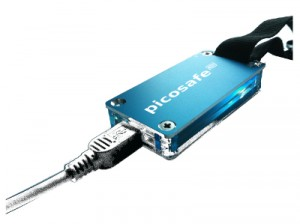
\includegraphics[width=0.35\textwidth]{picosafe_splash.png}
  \end{center}
  \caption{Picosafe USB stick.}
\end{wrapfigure}

Picosafe combines a small embedded linux device, secure booting and encrypted
root filesystem, and low power consumption.

The code of the bootloader is stored encrypted and only gets decrypted at
runtime. Starting from the bootloader a chain of trust is established by
validating each software component. The bootloader validates kernel and
initramfs and the initramfs will mount only an encrypted root filesystem.
Therefore only trusted software will run on picosafe.

Picosafe uses a 270 MHz LPC3143 with 192 kB internal SRAM, AES decryption unit,
memory management unit, USB 2.0 and random number generator. In addition
picosafe provides 32 MiB SDRAM, SD memory card both for application and data,
two LEDs and an USB device.

\section{Features}

\begin{itemize}
\item LPC3143
  \begin{itemize}
  \item 270 MHz, 32bit  ARM926EJ-S
  \item 16 kB D-cache and 16 kB I-cache
  \item memory management unit (MMU)
  \item 192 kB embedded SRAM
  \item AES decryption unit
  \item secure one-time programmable memory for AES key
  \item 128 bit unique id
  \item random number generator
  \item High-speed USB 2.0 (OTG, Host, Device) with on-chip PHY
  \item DMA controler
  \end{itemize}
\item 32 MB SDRAM
\item SD-card for applications and data
\item secure boot – established chain of trust at bootup
\item linux system
\item two LEDs (green and red)
\item small device
\item low power consumption
\end{itemize}

\section{Security Concept}

Picosafe's LPC3143 will only load encrypted code after reset. In order to run
any code after reset (typically the bootloader), the code must be correctly
encrypted with a 128 bit AES key. The AES key is stored in the OTP area of the
LPC3143 and different for every picosafe device.

In order to establish a chain of trust, every software component must validate
the next software component, i.e. the bootloader must validate kernel and
initramfs, initramfs must validate the root filesystem.

Following steps are performed:
\begin{enumerate}
\item LPC3143 loads bootloader from SD-card
\item LPC3143 decrypts bootloader with AES key stored in OTP area
\item LPC3143 executes decrypted bootloader
\item apex bootloader loads and validates kernel and initramfs:
  \begin{itemize}
  \item Possibility 1: Encrypting bootloader

  Kernel and initramfs are encrypted with the same AES key the LPC3143 uses to
  decrypt the bootloader. The apex bootloader loads kernel and initramfs from
  the SD-card and decrypts both. The bootloader will also check if the decrypted
  data contains a certain magic string to verify that the kernel is valid.

  \item Possibility 2: Verifying signature

  Kernel and initramfs are signed. The apex bootloader contains a public key
  (RSA 1024bit) that can be used to verify the signature of kernel and
  initramfs. The apex bootloader loads kernel and initramfs, calculates the
  SHA-1 checksum and verifes the signature. If verification was not successful,
  the memory area of kernel and initramfs will be overwritten with zeroes.
  \end{itemize}
\item The kernel boots up, initializes hardware and executes \texttt{init} on the
initramfs. \texttt{init} sets up a network connection over USB and starts a webserver. The user can insert the
password of the root-filesystem on a SSL secured webpage.
\item If the user provides the correct password, the root-filesystem can be mounted and the linux system starts.
\item The user can log in via ssh or use other services of the system such as webserver, databases etc.
\end{enumerate}

The user may modify software components to meet demands. Configuring and
customizing bootloader, kernel and initramfs, and root-filesystem are described
in the corresponding chapters.

\begin{figure}
  \begin{center}
    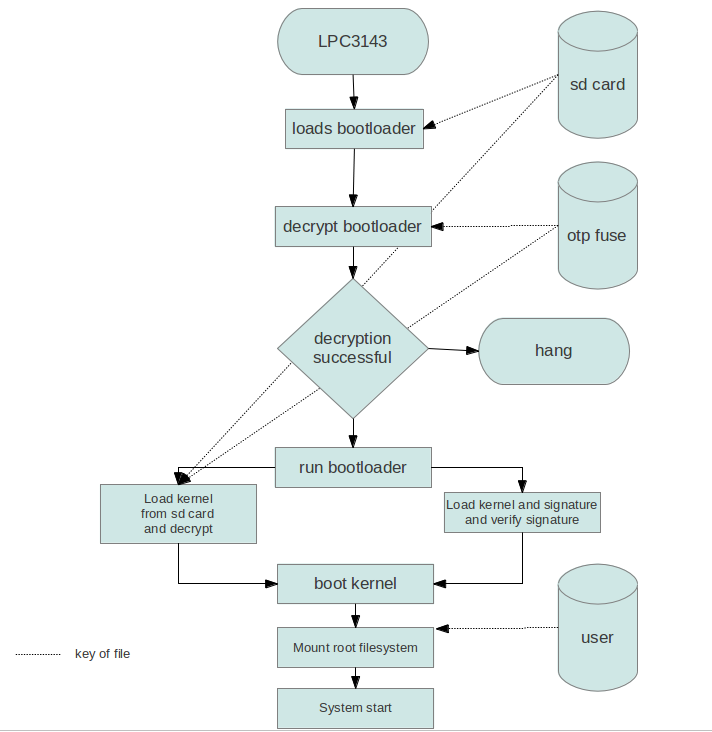
\includegraphics[width=0.6\textwidth]{diagram_key_files_flow.png}
  \end{center}
  \caption{Flowchart of boot process.}
\end{figure}

\subsection{Encrypted/protected data/code}

The boot process of the linux system consists of three different parts of software:
\begin{enumerate}
\item bootloader
\item kernel and initramfs
\item root-filesystem
\end{enumerate}

The bootloader is encrypted. The AES key is stored in the OTP memory of the
LPC3143 and cannot be read out.

An attacker may overwrite the bootloader on the sd-card with arbitrary data.
But the LPC3143 will first decrypt the data and then execute the code. As the
attacker doesn't know the AES key, the LPC3143 will execute random and probably
invalid code.

For kernel and initramfs there are two possibilities:
\begin{enumerate}
\item Kernel and initramfs may be encrypted in the same way the bootloader is
encrypted. Then the same arguments apply.
\item Kernel and initramfs are not encrypted, but the bootloader checks the
signature of kernel and initramfs. If so, an attacker may read kernel and
initramfs (e.g. secret strings or the configuration of the kernel), but cannot
change kernel or initramfs.
\end{enumerate}

The initramfs mounts the root-filesystem. To do so, the user has to insert a
password to mount the root-filesystem. The root-filesystem will only open, if
the supplied password is correct. So if the root-filesystems can be mounted,
the files on the root-filesystem haven't been altered. (Please notice that an
attacker may destroy data – e.g. by overwriting the root-filesystem or simply
by breaking the SD-card into pieces.)

\subsection{Unencrypted/unprotected data/code}

Picosafe validates the integrity of bootloader, kernel and initramfs and
root-filesystem. However, the SDRAM is not encrypted. An attacker may read the
SDRAM at runtime or even modify e.g. kernel code in the SDRAM at run time. This
is not a trivial attack, but it can be done. Also be aware of cold boot
attacks! The content of the SDRAM will not magically vanish after shutdown. An
attacker may read out data from the SDRAM even after poweroff!

As a precaution, you may
\begin{itemize}
\item Encrypt RAM:

This is possible by creating a RAM disk with encrypted filesystem that contains
a swap file. However, not all memory will be stored in the encrypted swap file,
the key will be stored in plain text somewhere in the memory and the kernel
code will not be encrypted at all. This will make attacks a bit harder, but it
won't fix the problem.
\item Clear RAM before poweroff:

This will prevent cold boot attacks. However, you cannot ensure that you can
always overwrite the RAM before poweroff. Also an attacker may still read and
modify the RAM during runtime.
\item Store sensible data in the internal SRAM of the LPC3143:

For very sensible data you may use the internal SRAM of the LPC3143. However,
you can only access this memory in kernel mode and you have to be very careful
that your data doesn't get stored in the SDRAM as well. Also, you only have 192
kB of SRAM!
\item Use emulation:

You may adjust/write an emulator that emulates an ARM device and encrypts the
external SD-RAM. This will decreace performance drastically, it will take some
time to adjust/write such an emulator, but it will certainly fix the security
problem.
\end{itemize}

\section{About this document}

\begin{itemize}
\item This document explains how the components bootloader, kernel, initramfs and root-filesystem can be compiled/generated and modified.
\item This document assumes that you are using a Ubuntu 12.04 system on a 32-bit x86 system. However, most of the document should apply to all linux distrubutions.
\item This document also assumes that you have basic experience in using linux and a linux shell like bash.
\item If you find mistakes, please send us a mail to \href{mailto:picosafe@embedded-projects.net}{picosafe@embedded-projects.net}.
\end{itemize}

